\chapter{Zasada działania sterownika układu}

W niniejszym rozdziale zaprezentowano opis działania sterownika układu. Zdefiniowano wymagania dotyczące pracy każdego z czterech trybów jazdy oraz przedstawiono sposób informowania użytkownika o aktualnym stanie, w którym znajduje się sterownik układu.
\newcolumntype{C}[1]{>{\centering}m{#1}}

\section{Struktura programu}

Cel projektu to wykonanie układu zmiany przełożeń, który oferuje dwa tryby pracy - tryb ręczny oraz automatyczny. Autor zdecydował, że w ramach trybu automatycznego wykonany zostanie podział na tryby: comfort, active i sport. Inspiracją  takiego rozwiązania jest branża motoryzacyjna, w której coraz częściej można spotkać układy automatycznej zmiany przełożeń, oferujące możliwość profilowania charakterystyki działania zmiany biegów, poprzez wybór jednego z trybów jazdy. 

Zasada działania programu przedstawiona została na rys. \ref{fig:schematAlgorytmu} i może być porównana do zasady działania skończonej maszyny stanów. Maszyna stanów jest pojęciem abstrakcyjnym, które definiuje zachowanie systemu jako skończony zbiór stanów oraz przejść pomiędzy stanami. Autor rozważał wykorzystanie systemu czasu rzeczywistego freeRTOS, w którym poszczególne stany będą odpowiadały nowym zadaniom, odpalanym sekwencyjnie. Jednak właśnie ze względu na sekwencyjne wykonywanie głównych zadań oraz brak ostrych wymagań czasowych, pomysł ten został odrzucony. Program działa na prostej zasadzie pętli nieskończonej, w której poszczególne zadania wyzwalane są przez układy czasowo-licznikowe. Dlatego porównanie programu do skończonej maszyny stanów odnosi się jedynie do wysokopoziomowego opisu zasady działania kontrolera. 

Cztery stany odpowiadają zaprojektowanym trybom jazdy - tryb ręczny, comfort, active oraz sport. Przejścia pomiędzy tymi stanami następują w wyniku naciśnięcia przycisku zmiany aktualnego trybu jazdy. Kolejność przejść przedstawiona została na rys. \ref{fig:schematAlgorytmu}. Wyróżnione zostały również trzy stany alarmowe: błąd komunikacji I2C, niski poziom naładowania pakietu zasilającego i rozładowanie pakietu zasilającego. 
\begin{figure}[h]
    \centering
    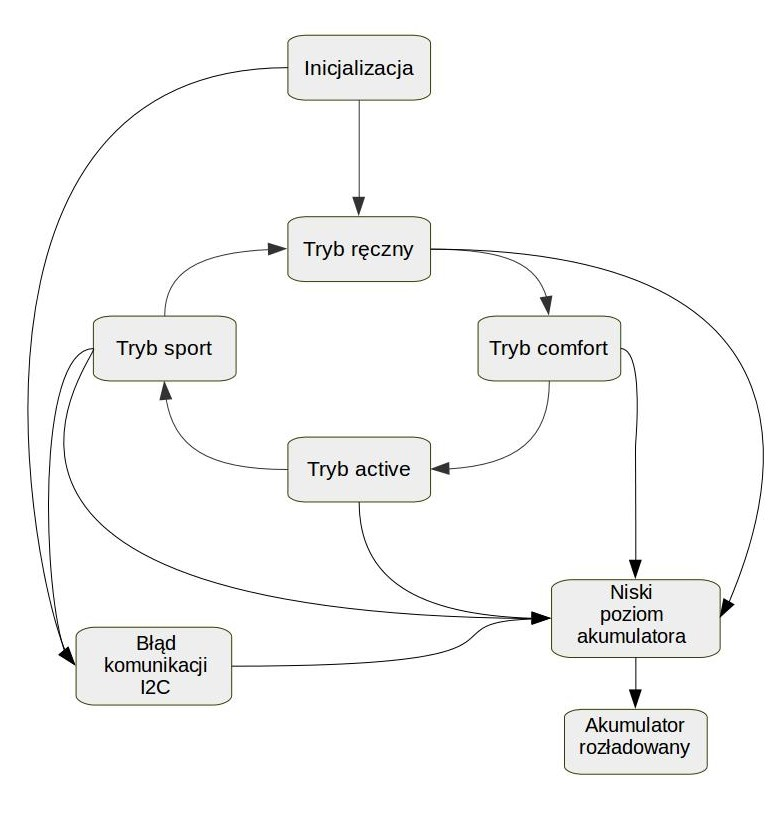
\includegraphics[scale=0.42]{schematAlgorytmu.jpg}
    \caption{Schemat ilustrujący zasadę działania programu kontrolera.}
    \label{fig:schematAlgorytmu}
\end{figure}
%_____________________________________________________________________________________________________________
\section{Opis stanów programu}
\subsection{Inicjalizacja układów peryferyjnych mikrokontrolera}
Stan inicjalizacji jest stanem początkowym programu, osiąganym jednokrotnie, po włączeniu zasilania. W tym stanie przeprowadzana jest inicjalizacja następujących układów peryferyjnych:
\begin{itemize}
\item
Porty wejściowe odpowiedzialne za obsługę przycisków do zmiany przełożeń oraz czujników magnetycznych.
\item
Porty wyjściowe odpowiedzialne za generowanie sygnału sterującego serwomechanizmem oraz sterowanie wskaźnikiem RGB aktualnego stanu programu. 
\item
Inercyjna jednostka pomiarowa.
\item
Układy czasowo licznikowe, które inicjują zadania okresowe oraz wykorzystywane są do pomiaru prędkości obrotowej i kadencji.
\end{itemize}

W przypadku, gdy inicjalizacja wszystkich układów przebiegnie bez błędów, następuje przejście do następnego stanu - tryb ręczny. Jeśli inicjalizacja jednostki pomiarowej IMU nie powiedzie się, zgłaszany jest błąd komunikacji I2C. 
%_____________________________________________________________________________________________________________
\subsection{Tryb ręczny}
Tryb ręczny jest pierwszym stanem, w którym użytkownik może korzystać z funkcjonalności układu zmiany przełożeń. Zasada działania odpowiada w pełni mechanicznemu układowi. W tym trybie obsługiwane są jedynie przyciski do zmiany przełożeń. Oprogramowanie umożliwia jednokrotną zmianę przełożenia, aktywowaną poprzez naciśnięcie odpowiedniego przycisku. Dodatkowo zaimplementowana została ciągła zmiana przełożeń, która uruchamiana jest poprzez naciśnięcie i przytrzymanie odpowiedniego przycisku. Przełożenia zmieniane są co 0.7 sekundy, więc użytkownik ma odpowiednio dużo czasu do zatrzymania zmiany na odpowiednim przełożeniu.

Naciśnięcie przycisku zmiany trybu pracy układu powoduje przejście do kolejnego stanu - trybu comfort.
%_____________________________________________________________________________________________________________
\subsection{Tryb comfort}
Stan comfort odpowiada pierwszemu z zaimplementowanych trybów automatycznej zmiany przełożeń. Ten tryb jest przeznaczony do spokojnego przemieszczania się na rowerze po płaskim terenie. Jest to najprostszy z trybów automatycznych, w którym użytkownik nie powinien angażować się w podejmowanie wyboru przełożenia. Możliwość zmiany ręcznej jest wyłączona. Mierzona jest jedynie chwilowa wartość kadencji. Płaski charakter trasy sprawia, że cykliczne zadanie, w trakcie którego dobierane jest przełożenie, zależne od wartości kadencji, uruchamiane jest z niską częstotliwością. Zakres kadencji jest stały dla każdego przełożenia i dobrany w taki sposób, aby umożliwić spokojną i komfortową jazdę na rowerze. W trakcie przejazdów testowych Autor uznał, iż jazda komfortowa odpowiada utrzymaniu kadencji w zakresie od $45$ do $60$ obrotów na minutę.
%_____________________________________________________________________________________________________________
\subsection{Tryb active}
Stan active odpowiada drugiem z zaimplementowanych trybów automatycznej zmiany przełożeń. Autor założył, iż ten tryb powinien być używany na trasach o zróżnicowanej topografii terenu. Dlatego zadanie cykliczne dla tego trybu uruchamiane jest z większą częstotliwością, niż w przypadku trybu comfort - raz na dwie sekundy. Zakres kadencji jest stały dla każdego przełożenia. Ze względu na zmienną topografię terenu, został rozszerzony względem trybu comfort i wynosi od $55$ do $70$ obrotów na minutę. Możliwa jest również ręczna zmiana przełożeń, która wskazuje na chęć przejęcia kontroli nad przełożeniami przez użytkownika. W takiej sytuacji zadanie cykliczne wyłączane jest na $10$ sekund. W tym czasie kontroler nie ma wpływu na dobór przełożeń. W tym trybie brana pod uwagę jest również chwilowa wartość prędkość roweru. Jeśli zostanie wykryty brak obrotów mechanizmu korbowego, następuje automatyczny dobór przełożenia, zgodny z tabelą \ref{tab:zakresOdPredkosci}, które zostanie ustawione w momencie wznowienia pedałowania. Ma to na celu umożliwienie zmiany o kilka przełożeń w przypadku, gdy rozpoczął się zjazd, a użytkownik przerwał pedałowanie. Ponowne wznowienie pedałowania skutkuje natychmiastowym doborem przełożenia dostosowanym do aktualnej prędkości, bez potrzeby przechodzenia przez poszczególne biegi. 
\begin{table}[h]
    \caption{Związek pomiędzy zakresem prędkości a przełożeniem dobieranym po wznowieniu pedałowania.}
    \begin{center}
		\label{tab:zakresOdPredkosci}
		\begin{tabular}{|c|c|c|c|c|c|c|c|c|}
 			\hline
 			\textbf{Zakres prędkości} $[\frac{km}{h}]$ & [0,2) & [2, 5) & [5,10) & [10,14) & [14,18) & [18,22) & [22,26) & [26, 100] \\
 			\hline
 			\textbf{Nr przełożenia} & 1 & 2 & 3 & 4 & 5 & 6 & 7 & 8 \\
			\hline
		\end{tabular}
	\end{center}
\end{table}
%_____________________________________________________________________________________________________________

\subsection{Tryb sport}  
Stan sport odpowiada ostatniemu z zaimplementowanych trybów automatycznej zmiany przełożeń. Tryb ten powinien być używany w trakcie bardzo dynamicznej jazdy na rowerze, której celem jest przejechanie danej trasy w bardzo szybkim tempie. Zadanie cykliczne tego trybu jazdy uruchamiane jest z taką samą częstotliwością, jak w przypadku trybu active. Autor podjął taką decyzję, ponieważ uważa, iż częstsze zmiany przełożeń w rowerze są nieefektywne. Zamiast skupić się na generowaniu mocy, użytkownik skupia się na szybkiej pracy układu zmiany przełożeń. Tak jak w trybie active, możliwa jest ręczna zmiana przełożeń, która implikuje wyłączenie kontrolera na $10$ sekund. Przełożenia dobierane są w zależności od wartości kadencji. W przeciwieństwie do pozostałych trybów, zakresy kadencji nie są stałe. Powstało wiele prac poruszających zagadnienie doboru optymalnej kadencji w kolarstwie \cite{cuttingEdge}, \cite{optCadence}. Ze względu na mnogość wskaźników jakości przyjętych w trakcie przeprowadzonych badań, zróżnicowaną charakterystykę poszczególnych wyścigów czy personalne predyspozycje zawodników, nie można wyznaczyć jednej wartości optymalnej dla wszystkich przypadków. Jednak wskazuje się na to \cite{cuttingEdge}, że zakres kadencji na odcinkach płaskich, wynoszący od 80 do 100 obrotów na minutę, pozwala zachować odpowiedni kompromis pomiędzy osiągami a wydajnością zawodnika. W przypadku podjazdów zaleca się obniżenie kadencji do około 70 obrotów na minutę. Są to zalecenia dotyczące kolarzy zawodowych, których osiągi znacznie przewyższają możliwości normalnych użytkowników. Zdecydowano, że zakresy kadencji w trybie sport będą uzależnione od kąta nachylenia terenu trasy rowerowej i zostaną obniżone względem wartości wymienianych w literaturze. Rozróżniane zatem są 3 możliwości doboru zadanej kadencji:
\begin{itemize}
\item
Nachylenie terenu jest mniejsze niż $-3^{\circ}$. Oznacza to zjazd ze zbocza o nachyleniu większym, bądź równym 5\%. Zakres kadencji jest obniżony względem jazdy po płaskim terenie i wynosi od 55 do 70 obrotów na minutę.
\item
    Nachylenie terenu należy do zakresu od $-3^{\circ}$ do $3^{\circ}$. Oznacza to jazdę po względnie płaskim terenie. Zakres kadencji wynosi od 70 do 85 obrotów na minutę.
\item
Nachylenie terenu jest większe niż $3^{\circ}$. Oznacza to podjazd pod zbocze o nachyleniu większym bądź równym 5\%. Zakres kadencji jest podwyższony względem jazdy po płaskim terenie i wynosi od 55 do 70 obrotów na minutę.

\end{itemize}
%______________________________________________________________________________________________________________
\subsection{Błąd komunikacji I2C}
Przejście do tego stanu może nastąpić w dwóch przypadkach. Pierwszy z nich to problemy z komunikacją w trakcie inicjalizacji jednostki pomiarowej wynikające z braku fizycznego połączenia pomiędzy jednostką pomiarową a portami mikrokontrolera. Drugi to problemy związane z odczytem danych w trybie sport. W tym przypadku może również dojść do problemów z komunikacją. Druga przyczyną mogą być niepoprawne wartości zwracane przez czujniki, świadczące o ich uszkodzeniu.

Problemy z komunikacją objawiają się brakiem odpowiedzi jednostki pomiarowej na rozkazy wysyłane przez mikrokontroler. Przed każdą próbą komunikacji odpalany jest układ czasowo-licznikowy. Jeśli odpowiedź od jednostki przyjdzie w krótszym czasie, niż jedna sekunda po wysłaniu zapytania, układ mierzący czas jest wyłączany. W przeciwnym przypadku wykryty zostaje błąd komunikacji.  
%_____________________________________________________________________________________________________________
\subsection{Niski poziom oraz rozładowanie pakietu}
\label{niskiPoziom}
Obydwa stany odnoszą się do problemu z pakietem zasilającym. Niski poziom naładowania odnotowywany jest wtedy, gdy napięcie pakietu zasilającego spadnie poniżej 6.8V. Następuje wtedy ograniczenie funkcjonalności systemu w celu oszczędności energii. Program przechodzi do stanu ręcznej zmiany przełożeń. Tryby automatycznej zmiany zostają wyłączone. W efekcie nie są obsługiwane żadne czujniki pomiarowe.

Jeśli napięcie pakietu zasilającego spadnie poniżej 6V, kontroler przechodzi w tryb pracy z rozładowanym pakietem zasilającym. Jest to tryb maksymalnej oszczędności energii. Wyłączona zostaje możliwość zmiany przełożeń. Działa jedynie dioda RGB sygnalizująca rozładowanie pakietu.

Autor zakłada, że następstwem osiągnięcia tych stanów jest naładowanie pakietu zasilającego. Nie ma zatem możliwości powrotu z tych stanów do normalnej pracy układu. Tak samo dzieje się w przypadku problemów z jednostką pomiarową.

\begin{table}[h]
    \caption{Kodowanie stanu programu w postaci kolorów RGB}
    \begin{center}
		\label{tab:rgb}
		\begin{tabular}{|c|c|}
			\hline
 			\textbf{Stan programu} & \textbf{Kolor RGB}\\
 			\hline
 			Inicjalizacja & biały\\  
 			\hline
			Tryb ręczny & żółty\\
			\hline
			Tryb comfort & zielony \\  
			\hline
			Tryb active & niebieski\\  
			\hline
			Tryb sport & różowy \\  
			\hline
			Niski poziom naładowania pakietu & czerwony migający\\  
			\hline
			Pakiet rozładowany & czerwony \\  
			\hline
			Błąd komunikacji I2C & biały migający\\  
			\hline
		\end{tabular}
	\end{center}
\end{table}
%______________________________________________________________________________________________________________
\subsection{Wskaźnik aktualnego trybu}

Wskaźnik aktualnego stanu, w którym znajduje się kontroler, jest istotnym elementem układu. Umożliwia  użytkownikowi sprawdzenie aktualnego trybu jazdy oraz informuje o stanach alarmowych. Autor uznał, iż dobrym wskaźnikiem aktualnego stanu będzie dioda RGB, która pozwala na zakodowanie wszystkich stanów w postaci odpowiednich kolorów. Taka reprezentacja stanów, w porównaniu np. do wyświetlacza, wydaje się być bardziej efektywna w trudnym terenie, gdzie rower narażony jest na duże wstrząsy i odczyt z ekrany mógłby zabrać więcej czasu. Do tego montaż prostej diody w okolicy kierownicy jest zdecydowanie prostszy i mniej narażony na uszkodzenia.
Kodowanie stanów w postaci kolorów diody RGB przedstawione zostało w tabeli \ref{tab:rgb}.


%______________________________________________________________________________________________________________

















